\chapter{The Recursion Theorem and Logic}

\section{Self-reproduction Paradox}

Suppose a Factory makes cars, meaning complexity of factory is greater than complexity of cars. But can a factory makes factories? 

Similarly, can a program print itself?(YES!)

\subsection{A self-reproducing TM}
\begin{theorem}
    There is a TM \(SELF\) which (on any input) halts with \(\langle SELF \rangle\) on the tape. 

    \begin{lemma}
        There is a computable function \(q: \Sigma^* \rightarrow \Sigma^*\) such that \(q(w) = \langle P_w \rangle \)  for every \(w\), where \(P_w\) is the TM \(P_w\) = "Print \(w\) on the tape and halt".

        (\(q(w)\) is the description of a TM \(P_w\) who prints \(w\) and halts.)
        \begin{note}
            Computable function \(f\) means if there is a TM \(M\) for all input \(w\), it halts with \(f(w)\) on the tape. 
        \end{note}      
    \end{lemma}
    \begin{proof}
        Straightforward, we can apparently make such kind of function.
    \end{proof}
\end{theorem}
\begin{proof}
    \(SELF\) has 2 parts, \(A\) and \(B\). 

    \(A\) = \(P_{\langle B \rangle}\), which makes \(A\) can print a \(\langle B \rangle\) on the tape:

    \begin{figure}[H]
        \centering
        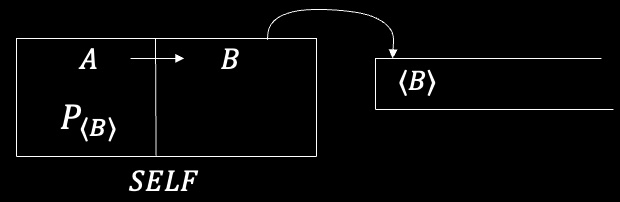
\includegraphics[width=0.6\textwidth]{l11.1.jpg}
        \caption{\(A\) print \(\langle B \rangle\) on the tape}
    \end{figure}

    \begin{intuition}
        Can we also do the same in \(B\) and makes it print \(A\)? 

        No! Because this is circular reasoning, \(A\) contains the serialization form of \(B\), if \(B\) contains the serialization form of \(A\), then the machine will be infinite large.
    \end{intuition}

    \(B =\) \begin{enumerate}
        \item "Compute \(q(tape :;contents)\)  to get \(A\) (The tape content happens to be \(\langle B \rangle\), but it does not care) 
        \item Combine with \(B\) to get \(AB = SELF\)
        \item Halt with \(\langle SELF \rangle\) on tape."   
    \end{enumerate} 

    \begin{figure}[H]
        \centering
        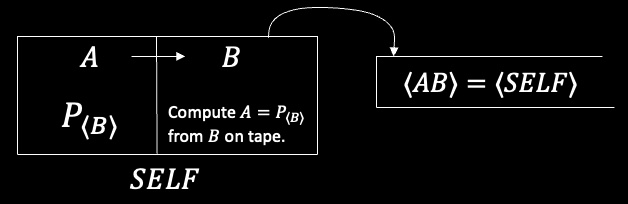
\includegraphics[width=0.6\textwidth]{l11.2.jpg}
        \caption{Print \(\langle AB \rangle\) on the tape}
    \end{figure}
\end{proof}

\begin{example}[English Implementation]
    Write "Hello World":\\
    > \verb|Hello World|

    Write the following twice, the second time in quotes "Hello World":\\
    > \verb|Hello World "Hello World"|

    Write the following twice, the second time in quotes\\
    "Write the following twice, the second time in quotes":\\
    > \verb|Write the following twice, the second time in quotes|\\
    > \verb|"Write the following twice, the second time in quotes"|
\end{example}

The upper phrase of the English example is called \underline{Action} part, the \(B\) in the TM is the \underline{Action} part. 

\section{The Recursion Theorem}

\begin{theorem}[Compute your own description]
    Let \(T\) be a TM that computes a function \(t: \Sigma^* \times \Sigma^* \rightarrow \Sigma^*\). 
    There is a TM \(R\) that computes a function \(r:\Sigma^* \rightarrow \Sigma^*\), where for every \(w\),
    \[
        r(w) = t(\langle R \rangle, w)
    \]   
    \begin{remark}
        \(r\) works exactly like \(t\) except \(r\) provides the description of \(R\).    
    \end{remark}
\end{theorem}
\begin{proof}
    \(R\) has 3 parts: \(A\), \(B\) and \(T\).

    \(T\) is given. 

    \(A = P_{\langle BT \rangle}\) 

    \begin{figure}[H]
        \centering
        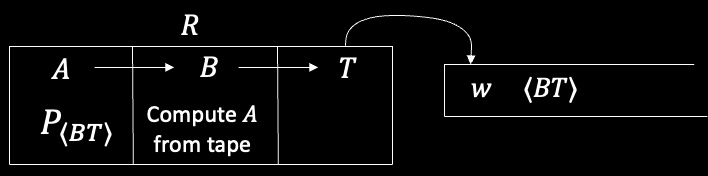
\includegraphics[width=0.6\textwidth]{l11.3.jpg}
        \caption{Print \(\langle BT \rangle\) on the tape}
    \end{figure}

    \(B = \) \begin{enumerate}
        \item "Compute \(q(tape :; contents :; after:; w)\) to get \(A\)
        \item Combine with \(BT\) to get \(ABT = R\)
        \item Pass control to \(T\) on input \(\langle w, R \rangle\)."      
    \end{enumerate} 

    \begin{figure}[H]
        \centering
        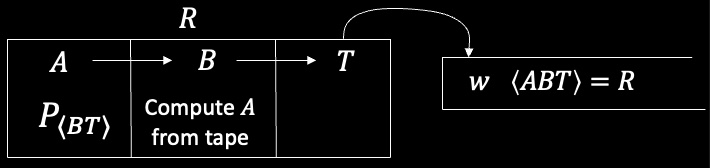
\includegraphics[width=0.6\textwidth]{l11.4.jpg}
        \caption{Print \(\langle ABT \rangle\) on the tape}
    \end{figure}
\end{proof}

\begin{note}
    The recursion theorem provides the ability to implement the self-referential \(this\) into any programming language. 
    With it, any program has the ability to refer to its own description, which has certain applications.
\end{note}

\subsection{\(A_{TM}\) is undecidable - new proof}
\hyperref[theorem: A(TM) not decidable]{\(A_{TM}\) is not decidable} is a very important conclusion, we used it to prove halting theorem.

\begin{theorem}
    \(A_{TM}\) is not decidable. 
\end{theorem}
\begin{proof}
    Assume some TM \(H\) decides \(A_{TM}\). 

    Consider the following TM \(R\):
    \(R\) = "On input \(w\)
    \begin{enumerate}
        \item Get own description \(\langle R \rangle\) (This is the content of the recursion theorem!)
        \item Use \(H\) on input \(\langle R, w \rangle\)  to determine whether \(R\) accepts \(w\) (This is the definition of \(A_{TM}\), our assumption is that \(R\) can decide whether any TM can accept any input)
        \item Do the opposite of what \(H\) says"
    \end{enumerate}   

    Suppose \(H\) reject \(\langle R, w \rangle\), \(R\) will accept the input \(w\). 

    We can rephrase this into: if \(R\) reject \(w\), \(R\) will accept \(w\): contradiction!     
\end{proof}
    

\subsection{Fixed-point Theorem}
    A \textbf{fixed point} of a function is a value that isn't changed by the application of the function.  
\subsection{\(MIN_{TM}\) is T-unrecognizable}

Other applications:
\begin{enumerate}
    \item Computer viruses
\end{enumerate}

\section{Intro to Mathematical Logic}
\begin{definition}[Goal]
    
\end{definition}


\begin{example}[A True but unprovable statement]
    
\end{example}

